\section{Introduction}
In the landscape of modern energy systems, generation technologies play a crucial role in shaping the way we harness and utilize power. From traditional fossil fuel-based methods to cutting-edge renewable sources, Generation technologies encompass a wide spectrum of solutions that drive the transition toward sustainable and efficient energy production. This section delves into the diverse range of generation and storage technologies, exploring their mechanisms, advantages, and challenges, while highlighting the pivotal role they play in shaping our energy future. Microgrids integrate these diverse renewable energy sources and storage into a functional system. Furthermore, Strategies for efficiently integrating RES and ES are also discussed and finally the proposed study on the energy management system is presented.\par
\section{Generation Technologies}
The first form of electricity generation was demonstrated by Thales when he rubbed amber with animal fur, although he attributed the objects to having some sort of soul \cite{6}. William Gilbert was the first person to use the term ‘Electricity’ in the late 1600s, over a lot of other invention related to electricity took place. In the early years of the 19th century that the works of Alessandro volta, Benjamin Franklin, Michael Faraday and Andre Ampere that really contributed to the electricity generating technologies we use today.\par
\subsection{DC and AC generation}
The development of Alternator and Dynamo paved the way for electricity power industry. The dynamo which produces DC electricity was developed by Werner Siemens and Charles Wheatstone in 1867. Electric motor, rotary converter and an alternator which generates AC electricity are all based on Dynamo.\par
Today it is common knowledge that alternators, commonly referred to as generators are preferred for electricity generations over Dynamos because alternating current distribution of power over large distances is more efficient than direct current. The first power station to have been built was in Bavarian town in 1878, it used steam to drive dynamos and the first power station to use an alternator was built in the United Kingdom in the town Godalming. Other technologies that we used to drive the generator soon followed, this includes, Hydropower, ignition engines, wind power, nuclear power etc. \par
In the recent years there have been an increase emphasis on renewable energy as the non-renewable sources will not always be available, and their direct role they play in global warming crisis make them not viable option for future generation of electricity.  The growth of solar and wind power has caused a rise in distributed generation systems such as microgrids.\par
However, the PV output power is also affected by environmental factors such as clouds, rainy conditions, deposition of snow or dust on the panel surface and the geographical location of the PV plant where the plant is installed. In the absence of solar radiation or in the nighttime, the battery bank in a PV system is used as a power backup to the connected load. The batteries have their constraints, such as short lifetime and replacement requirements during project lifetime \cite{7}.\par
\subsection{DC Generation Technologies}
Direct current is produced by generators with commutators, fuel cells, rectifiers and photovoltaic cells. DC generators are rarely used in power plants due to extensive use of AC over DC in transmission lines. \cite{8}.  Photo voltaic arrays generate DC electricity in the presence of adequate sun radiation, in case where the sun radiation is inadequate, wind generation is utilized by using rectifiers.  M.S. Keerthana et al. \cite{9} demonstrated a dual source DC Microgrid by using wind and solar. \par
\subsubsection{Photovoltaic Panel}
When sunlight (photons) strikes the photovoltaic cells, it releases energy that frees electrons from the semiconductor material, generating an electric current. The flow of electrons creates a direct current (DC) electricity within each photovoltaic cell. Multiple cells are connected in series or parallel to achieve the desired voltage and current levels. The generated DC electricity from the individual cells is combined within the panel using wiring and junction boxes. These components connect the cells and allow the collected electricity to be routed to the panel's output terminals.
A Matlab/Simulink model of a PV cell equivalent is shown in figure below.\par
\begin{figure}[H]
	\centering
	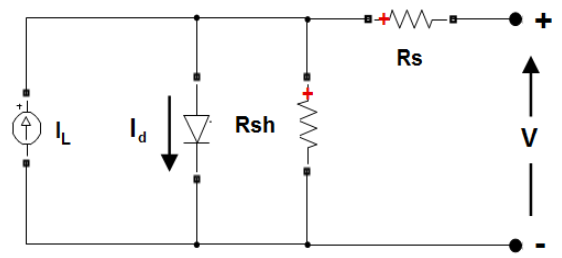
\includegraphics[totalheight=6cm]{Figures/pv cell.png}
	\caption{A Matlab/Simulink model of a PV cell}
	%	\label{fig:verticalcell}
\end{figure}
The voltage-current characteristic equations for the model above are defined as:
\begin{equation}
	{I_d}={I_o}(\exp(\frac{{V_d}}{{V_T}})-1)
\end{equation}
\begin{equation}
	{V_T}=\frac{{k_t}}{{q}}*nl*NCell
\end{equation}
Where:\par
\begin{list}{}{}
	\setlength\itemsep{-1em}
	\item ${I_d}$ = Diode current(A)
	\item ${V_d}$ = Diode voltage(V)
	\item ${I_o}$ = Diode saturation current(A)
	\item ${nl}$ = Diode ideality factor
	\item ${k}$ = Boltzman constant: 1.3806e-32 J.K-1
	\item ${q}$ = Electron charge: 1.6022e-19C
	\item ${T}$ =  Cell temperature (K)
	\item ${Ncell}$ = Number of cells connected in series in a module
\end{list}
The PV cells capture the energy of the sun and convert it into electricity. There are three main categories of PV panel options: Mono-crystalline solar panels, Poly-crystalline solar panels and thin-film solar panel.
\subsubsection{Poly-crystalline Panel}
Polycrystalline PV panels are made up of polycrystalline silicon produced from numerous mono-crystals. They are characterised by a light blue colour and distinctive crystal edges. Poly-crystalline photovoltaic panels are considered less efficient and more vulnerable to high temperatures. They are popular due to being less expensive than mono-crystalline Panels.
\subsubsection{Mono-crystalline Panel}
These panels use single-crystal silicon cells and are known for their high efficiency.
\subsubsection{Thin-film Panel}
Thin-film panels use various semiconductor materials deposited in thin layers on a substrate. They are flexible and can be used in diverse applications, but they typically have lower efficiency compared to crystalline panels.\par
In the assessment of various photovoltaic technologies, the researchers in \cite{10} determined that the performance of Mono-crystalline PV systems outperformed other technologies in terms of configuration. However, thin film systems have showed a slightly better performance in specific yield per installed capacity (1693 kWh/kWp) in comparison with Mono-crystalline (1678 kWh/kWp) due to its low temperature coefficient. Nevertheless, it is crucial to acknowledge that the effectiveness of a PV system is dependent upon a range of factors, including geographical location, installation angle, shading, maintenance, and cost considerations \cite{11}, \cite{12}.\par
\subsubsection{Thermoelectric generators (TEGs)} 
Thermoelectric generators convert heat into electricity by using the Seebeck effect. When there is a temperature difference between the two sides of the thermoelectric material, it creates an electric potential difference (voltage) between them. Electrons flow from the hot side to the cold side, generating an electric current. The generated electrical power is proportional to the temperature difference and the efficiency of the TEG.\par
TEGs have a very low efficiency and high cost \cite{13} which limits their application only in special areas. Search has been done to improve the TEG efficiency for applications in other areas such as \cite{14}. Unlike most DC generators, increasing (Thermal Energy Modules) TEMs does not linearly increase power generation capacity as stated by the authors in \cite{15}.\par
\subsubsection{Wind Turbine} 
A wind turbine is a device that converts the kinetic energy from the wind into mechanical energy and then transforms it to electricity. Wind turbines harness the power of the wind, and it is considered clean energy because no greenhouse gases are emitted during its operation. \par
A typical wind turbine consists of rotor blades, a tower, and a nacelle. The wind makes the blades spin and rotate a shaft connected to a generator \cite{16}. Wind turbines are inherently alternating current by nature. For use with other renewable energy sources such as PV, wind turbines must be converted to DC. 
\section{DC Distribution}
The DC distribution is the preferred topology for microgrid distribution systems. Nandini K.K. \cite{17} listed the following advantages of DC distribution system over AC:
\begin{itemize}
	\item The power factor is not necessary for calculating distribution loss in a DC system.
	\item The power losses associated with capacitance charging and discharging are eliminated.
	\item There is no requirement to consider utility grid synchronization or reactive power in the DC system.
	\item Battery converter primarily regulates the DC bus voltage using linear feedback. 
\end{itemize}
DC has its own disadvantages which include the lack of standardisations for LVDC distribution networks which were noted by, Katar et al \cite{18}. DC transmission lines has two basic distribution structures, the unipolar and bipolar system.
In a unipolar system figure 2.2, electric energy is carried over two voltage lines, the Vdc and 0Vdc for reference.
\begin{figure}[H]
	\centering
	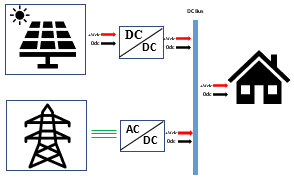
\includegraphics[totalheight=6cm]{Figures/unipolar grid.png}
	\caption{Uni-polar grid}
	%	\label{fig:verticalcell}
\end{figure}

The bipolar distribution system figure 2.3.2 carries three voltage lines, the +Vdc, the reference and the -Vdc.
\begin{figure}[H]
	\centering
	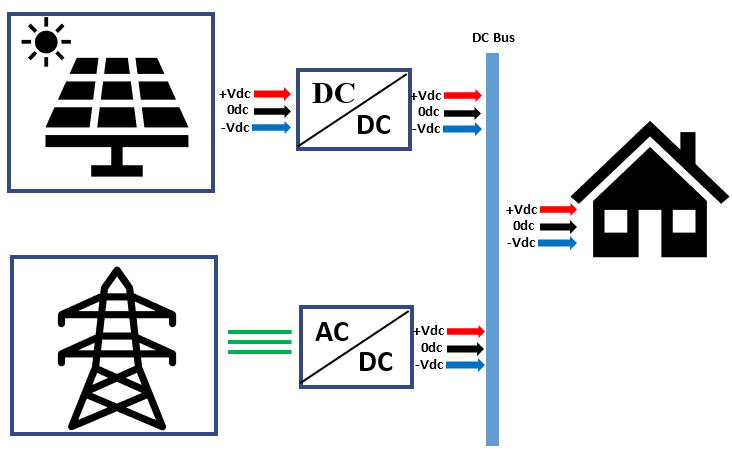
\includegraphics[totalheight=6cm]{Figures/bipolar grid.png}
	\caption{Bi-polar grid}
	%	\label{fig:verticalcell}
\end{figure}

\section{Energy Storage Technologies.}
Due to the intermittent nature of RES, which off-grid MG heavily relies upon, energy storage systems are used to power the grid when there is not enough sunlight for PV or wind speed to output the required energy to meet demand. 
There a many energies storage type, and each type can be further sub divided into categories. Table 2.1 below shows different types of energy storage systems:


\begin{center}
\begin{table}[!ht]
	\begin{center}
		\caption{Types of energy storage.}
		%\label{tab:table1}
		\begin{tabular}{|p{6cm}|p{8cm}|} % <-- Alignments: 1st column left, 2nd middle and 3rd right, with vertical lines in between
			\hline
			\textbf{Type of Energy Storage} & \textbf{Description and Applications}\\
			\hline
			Batteries & - Lithium-ion: Portable electronics, EVs\\
					  & - Lead-Acid: Automotive, backup power, renewables\\
					  & - Nickel-Metal Hydride: Hybrids, stationary\\
					  & - Flow Batteries: Grid-scale, scalability\\
					  & - Sodium-Ion: Grid-scale, emerging alternative\\
			\hline
			Pumped Hydroelectric Storage & - Water pumped to higher reservoir during low demand, released for peak\\
			\hline
			Compressed Air Energy Storage & - Compressed air stored, released through turbines\\
			\hline
			Flywheel Energy Storage & - Energy stored in rotational motion of flywheel\\
			\hline
			Thermal Energy Storage & - Heat or cold stored in materials for space heating, cooling\\
			\hline
			Hydrogen Energy Storage & - Electrolysis of water to produce hydrogen for power, transportation\\
			\hline
			Superconducting Magnetic & - Energy stored in superconducting coils, rapid discharge\\
			\hline
			Thermochemical Energy Storage & - Energy stored in chemical reactions, releases energy on demand\\
			\hline
			Electrochemical Capacitors & - High-power, quick charge and discharge\\
			\hline
			Gravitational Energy Storage & - Lifting weights for potential energy storage, releases for electricity\\
			\hline
		\end{tabular}
	\end{center}
\subsection{Electromechanical Storage} 
\end{table}
\end{center}

\begin{sloppypar}
Batteries represent the most prevalent form of energy storage and belong to the category of electromechanical storage solutions \cite{19}. Electromechanical storage involves conversion of chemical energy into electrical or vice versa through reduction-oxidation(redox) reactions. Batteries are electromechanical devices that store and release electrical energy through redox reaction. \par
\end{sloppypar}
A range of battery varieties are employed for energy storage purposes, encompassing lead acid batteries, lithium ion, sodium nickel chloride, nickel cadmium battery, etc. These batteries vary in their respective characteristics and application. \par
Renewable energy storage relies on various battery types to store excess energy generated from renewable sources like solar and wind. Lead acid battery are the oldest rechargeable batteries \cite{20}. They are well suited for application where reliability and cost are primary considerations. On the other spectrum Lithium ion is very costly however the make up in cost by their high energy density, efficiency, and life cycle.\par
\subsection{Hydrogen Energy Storage (HES)} 
Hydrogen energy storage uses hydrogen gas as a means to store and release energy. A fuel cell is used to store hydrogen energy. In a fuel cell hydrogen and oxygen react to form water to produce electricity. This method has gained attention as a versatile and potentially sustainable solution for addressing energy storage and distribution challenges. \par
their high energy density, efficiency, and life cycle.\par
\subsection{Mechanical Storage} 
Mechanical storage is the process of storing energy in mechanical systems and converting it back to usable energy when needed. The types of mechanical storage include pumped hydroelectric storage (PHD), Compressed Air Energy Storage (CAES), Flywheel Energy Storage, Gravitational Energy Storage. These types of energy storage have geographical and environmental constraints.\par
\subsection{Mechanical Storage} 
Supercapacitors use polarized liquid layers between conducting ionic electrolyte and conducting electrode to increase the capacitance. They have a very high energy density and power. Supercapacitors have a very low stage of charge compared to other electromechanical storage systems \cite{21}. They can be used to suppress power fluctuations in Wind and PV systems, they are generally combined with a battery system in a hybrid storage system.\par
\subsection{Thermal Energy Storage (TES)} 
Thermal energy storage is a method of storing thermal energy by heating or cooling and releasing it when needed. TES systems can also be used to mitigate the intermittent of renewable energy sources, by storing heat in water tanks, molten salts, or another material. \par
\section{Operational Strategies for DC Microgrids} 
There are two basic modes in which DC MGs are operated: Grid-connected and Off grid. Grid-connected in this instance means that the DC MG is connected to the utility, converters are used to convert from AC from the utility to DC used in DCMG transmission lines. EMS are integrated into MGs to improve efficiency and to maintain grid stability. In the absence of EMS control strategies for converters are used to improve grid performance.\par
Unlike the AC’s bus control systems which controls the AC bus voltage and frequency, The converters in DC microgrid have just one parameter to control, which is the DC bus voltage. \cite{22} discussed three control schemes used in DC microgrids: Constant-current control, constant voltage control, and droop control.\par
\subsection{Constant-current control} 
The constant-current control aims to keep the bus current at constant level and change in demand may greatly affect DC bus voltage. Energy storage systems can utilize the constant-current control strategy to help recover bus voltage in a short time.
\subsection{Constant-voltage control} 
This strategy aims to keep the voltage stable. Ultra-capacitors are used to reduce the fluctuations caused by changes in load demand.\par
\subsection{Droop control} 
The Droop control strategy is used to stabilize the voltage and solve the load sharing problem. \cite{22}. \cite{23} explained droop voltage using DC system voltage-current characteristic line (V-I characteristic line). The load demand will cause a change in the output current of converters, which will lead to the drop of bus voltage. The droop control scheme is the same as that of voltage-control, with the difference being reference voltage is replaced by droop voltage.\par
\begin{figure}[H]
	\centering
	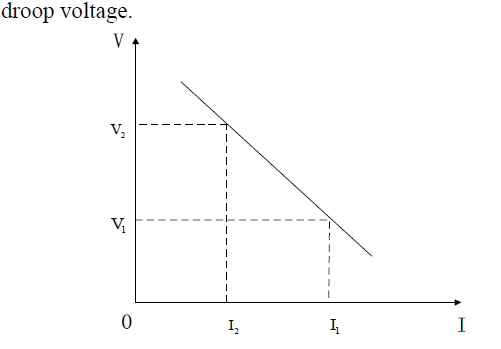
\includegraphics[totalheight=6cm]{Figures/dc voltage characteristics.png}
	\caption{DC voltage-current characteristic line}
	%	\label{fig:verticalcell}
\end{figure}
\section{Operational Strategies for DC Microgrids} 
Mohammed A.A et al \cite{24}, describes hierarchical control in their DCMG systems as consisting of three level; primary, secondary, and tertiary control.
\begin{enumerate}[nolistsep]
	\item Primary control deals with voltage/current regulation, and control of local power-sharing.
	\item Secondary control works on the top of primary control dealing with voltage compensation, power quality regulation, microgrid synchronization with any external grid, etc.
	\item Tertiary control is the highest level and is responsible for optimization, power management, economic dispatch, and overall system regulation.
\end{enumerate}
A communication less decentralised power-sharing method for composite storage devices developed by \cite{25}, their strategy allows plug and play of multiple batteries and ultracapacitors by implementing a master-slave control on additional batteries. This paper does not guarantee full equalisation of SoCs. Equalisation is highly dependent on load and power generation. \par
\section{EMS-integrated DC MG}
Energy Management Systems are used in MG to improve grid performance, reduce operational costs, and increase efficiency \cite{26}. Different algorithms for EMS have been proposed for different MG topologies.\cite{27} proposed a 4-level DC-based home management system to meet voltage levels of home appliances and devices. The EMS proposed in \cite{28} improves efficiency and power management by introducing three modes of operation: power mode, deficit, and power balance mode.\par
\section{Multi-level approach}
Multi agent systems in microgrids are made up of units called agents. From the MG perspective, agents are HEMS connected to it. The agent on the MG can be configured in two ways, centralised multi-agent coordination and de-centralised agent coordination. Figure 2.5 below illustrates the centralised multi-agent coordination described by \cite{29}, the coordinator is the central agent, it is responsible for commination between the agents.\par
\begin{figure}[H]
	\centering
	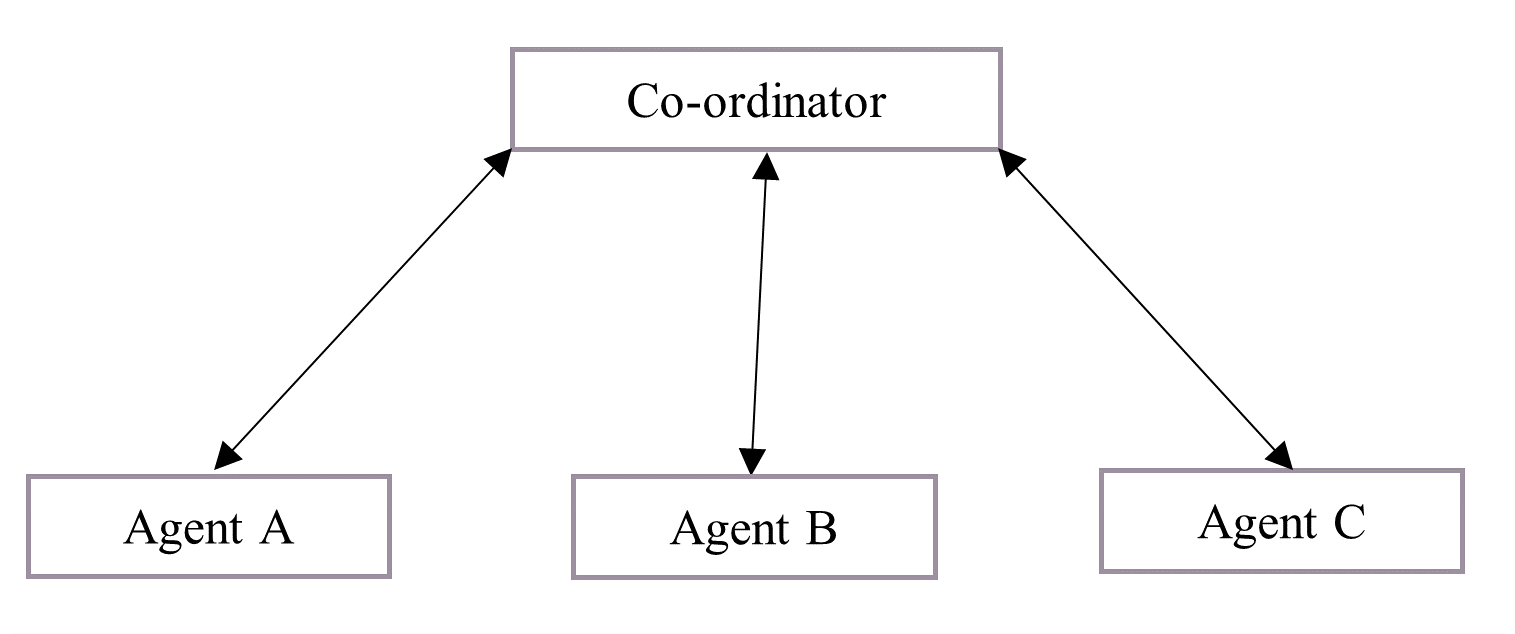
\includegraphics[totalheight=6cm]{Figures/centralised multiagent.png}
	\caption{Centralised multi-agent coordination}
	%	\label{fig:verticalcell}
\end{figure}
A de-centralized multi-agent co-ordination is shown below. In this architecture, the agents work independently, they communicate to each other to determine the status of other agents so they can perform the same task by associated motives.\par
\begin{figure}[H]
	\centering
	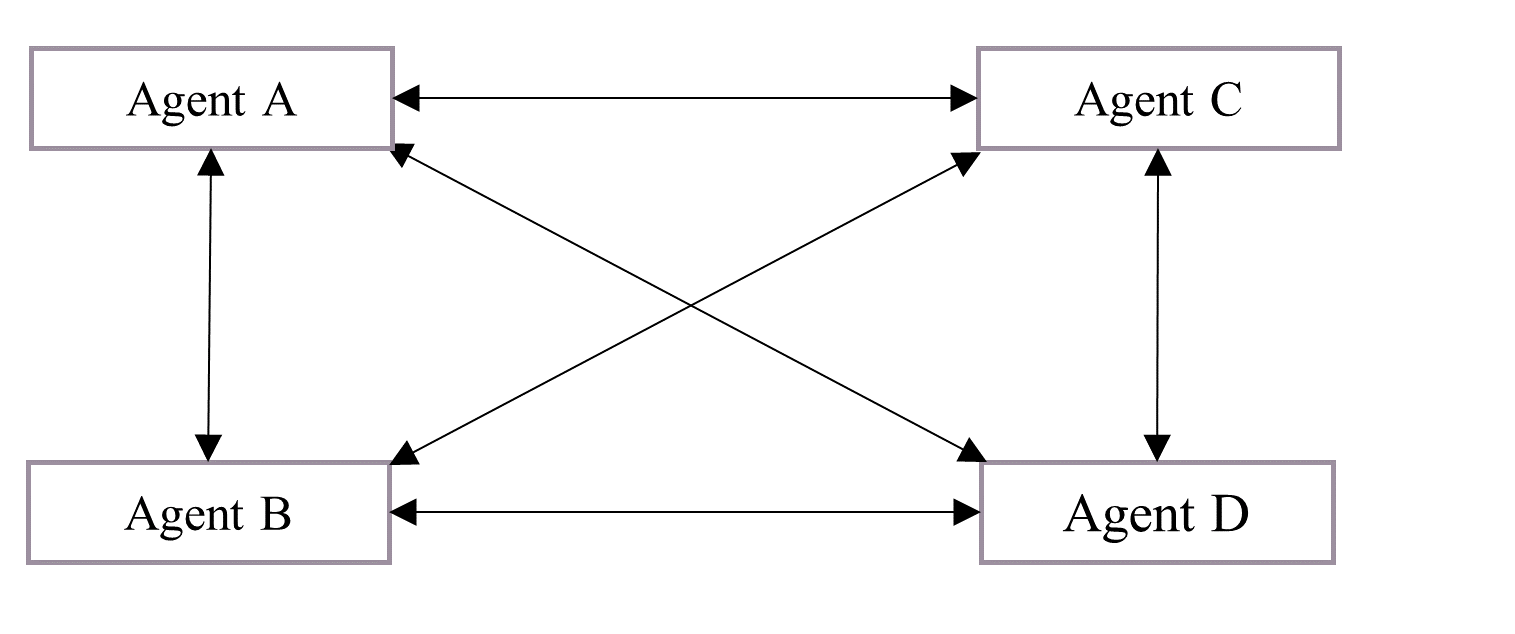
\includegraphics[totalheight=6cm]{Figures/decentralised multiagent.png}
	\caption{De-centralized multi-agent co-ordination}
	%	\label{fig:verticalcell}
\end{figure}
\section{Proposed study}
A microgrid can be defined as power cluster of distributed generation, load, and energy storage device accumulated together in the vicinity to each other \cite{30}. The most used distributed generation in residential areas are PV \cite{31}. The flexibility of the proposed EMS allows for residential units to be configured as DG, ESS, load, or any combination, depending on the resources available in the unit \cite{32}.\par
\subsection{Introduction}
Ahmad Alzahrani et al. \cite{32} described as a Systems of Systems (SoSs). SoSs are integrated systems that are diverse and autonomous but work together to achieve common goals. The systems can work together or independently. Table 1 below shows some characteristics of SoSs.
	\begin{table}[!ht]
		\begin{center}
			\caption{Systems of Systems characteristics}
			%\label{tab:table2}
			\begin{tabular}{|p{6cm}|p{8cm}|} % <-- Alignments: 1st column left, 2nd middle and 3rd right, with vertical lines in between
				\hline
				\textbf{Characteristic} & \textbf{Definition}\\
				\hline
				Operational Independence & All subsystems work independent and have no interference with other subsystems\\
				\hline
				Evolutionary development & Flexible to adding new subsystems\\
				\hline
				Emergent behaviour & The overall system works as collective unit to accomplish a big task\\
				\hline
				Geographic distribution & The subsystems are sequentially distributed to facilitate the flow of information\\
				\hline
				Managerial independence & The subsystems are in control of their own operation.\\
				\hline
			\end{tabular}
		\end{center}
	\end{table}
	
	From a microgrid layout, REMCS (Residential Energy Monitoring and Control systems) are systems that connect to another system such as CGMS (Central Grid Management system). REMCS subsystems capable of operating independently without any input or interference from CGMS. 
\subsection{Modelling the microgrid for the EMS using SoSs}
The SoSs have characteristics that allow easy integration of the EMS into the microgrid, with each system working independently, failure of one system will have little impact on the overall operation of the grid. Figure 5 below shows the DC microgrid connected to RES, loads and storage systems.\par
\begin{figure}[H]
	\centering
	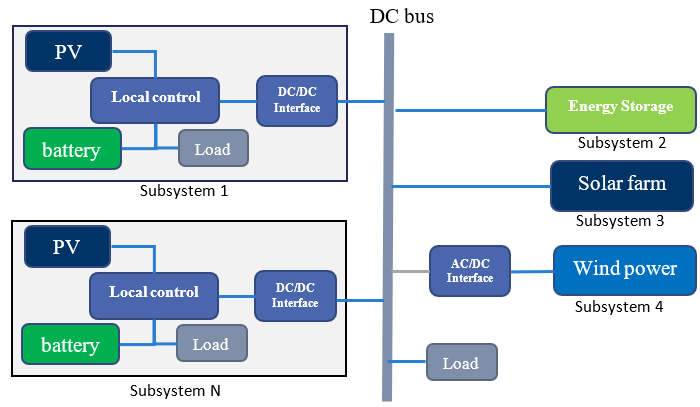
\includegraphics[totalheight=8cm]{Figures/dc mg systems of systems.png}
	\caption{DC MG Systems of Systems}
	%	\label{fig:verticalcell}
\end{figure}
\section{Conclusion}
This this section, energy generation, storage and distribution methodologies were reviewed to determine the best solution for DC MG application. From the studies above and taking account of all the cited references, energy management systems differ greatly due to grid attributes, such as centralised and decentralized, voltage regulation, frequency control, etc. \par
The current study proposes the adoption of a decentralized energy management system for the DC MG, characterized by a non-communicative framework. This approach capitalizes on the power sharing concept elucidated in reference  ,while additionally introducing a System of Systems framework to enhance control mechanisms and operational efficiency.\par
